% Options for packages loaded elsewhere
\PassOptionsToPackage{unicode}{hyperref}
\PassOptionsToPackage{hyphens}{url}
%
\documentclass[
]{article}
\title{enrichmotifpairR: An R package/shiny app for finding enriched
transcription factor motifs and their binding partners}
\author{Naresh Doni Jayavelu, Nicholas Moss, and R. David Hawkins}
\date{04/13/2022}

\usepackage{amsmath,amssymb}
\usepackage{lmodern}
\usepackage{iftex}
\ifPDFTeX
  \usepackage[T1]{fontenc}
  \usepackage[utf8]{inputenc}
  \usepackage{textcomp} % provide euro and other symbols
\else % if luatex or xetex
  \usepackage{unicode-math}
  \defaultfontfeatures{Scale=MatchLowercase}
  \defaultfontfeatures[\rmfamily]{Ligatures=TeX,Scale=1}
\fi
% Use upquote if available, for straight quotes in verbatim environments
\IfFileExists{upquote.sty}{\usepackage{upquote}}{}
\IfFileExists{microtype.sty}{% use microtype if available
  \usepackage[]{microtype}
  \UseMicrotypeSet[protrusion]{basicmath} % disable protrusion for tt fonts
}{}
\makeatletter
\@ifundefined{KOMAClassName}{% if non-KOMA class
  \IfFileExists{parskip.sty}{%
    \usepackage{parskip}
  }{% else
    \setlength{\parindent}{0pt}
    \setlength{\parskip}{6pt plus 2pt minus 1pt}}
}{% if KOMA class
  \KOMAoptions{parskip=half}}
\makeatother
\usepackage{xcolor}
\IfFileExists{xurl.sty}{\usepackage{xurl}}{} % add URL line breaks if available
\IfFileExists{bookmark.sty}{\usepackage{bookmark}}{\usepackage{hyperref}}
\hypersetup{
  pdftitle={enrichmotifpairR: An R package/shiny app for finding enriched transcription factor motifs and their binding partners},
  pdfauthor={Naresh Doni Jayavelu, Nicholas Moss, and R. David Hawkins},
  hidelinks,
  pdfcreator={LaTeX via pandoc}}
\urlstyle{same} % disable monospaced font for URLs
\usepackage[margin=1in]{geometry}
\usepackage{color}
\usepackage{fancyvrb}
\newcommand{\VerbBar}{|}
\newcommand{\VERB}{\Verb[commandchars=\\\{\}]}
\DefineVerbatimEnvironment{Highlighting}{Verbatim}{commandchars=\\\{\}}
% Add ',fontsize=\small' for more characters per line
\newenvironment{Shaded}{}{}
\newcommand{\AlertTok}[1]{\textcolor[rgb]{1.00,0.00,0.00}{\textbf{#1}}}
\newcommand{\AnnotationTok}[1]{\textcolor[rgb]{0.38,0.63,0.69}{\textbf{\textit{#1}}}}
\newcommand{\AttributeTok}[1]{\textcolor[rgb]{0.49,0.56,0.16}{#1}}
\newcommand{\BaseNTok}[1]{\textcolor[rgb]{0.25,0.63,0.44}{#1}}
\newcommand{\BuiltInTok}[1]{#1}
\newcommand{\CharTok}[1]{\textcolor[rgb]{0.25,0.44,0.63}{#1}}
\newcommand{\CommentTok}[1]{\textcolor[rgb]{0.38,0.63,0.69}{\textit{#1}}}
\newcommand{\CommentVarTok}[1]{\textcolor[rgb]{0.38,0.63,0.69}{\textbf{\textit{#1}}}}
\newcommand{\ConstantTok}[1]{\textcolor[rgb]{0.53,0.00,0.00}{#1}}
\newcommand{\ControlFlowTok}[1]{\textcolor[rgb]{0.00,0.44,0.13}{\textbf{#1}}}
\newcommand{\DataTypeTok}[1]{\textcolor[rgb]{0.56,0.13,0.00}{#1}}
\newcommand{\DecValTok}[1]{\textcolor[rgb]{0.25,0.63,0.44}{#1}}
\newcommand{\DocumentationTok}[1]{\textcolor[rgb]{0.73,0.13,0.13}{\textit{#1}}}
\newcommand{\ErrorTok}[1]{\textcolor[rgb]{1.00,0.00,0.00}{\textbf{#1}}}
\newcommand{\ExtensionTok}[1]{#1}
\newcommand{\FloatTok}[1]{\textcolor[rgb]{0.25,0.63,0.44}{#1}}
\newcommand{\FunctionTok}[1]{\textcolor[rgb]{0.02,0.16,0.49}{#1}}
\newcommand{\ImportTok}[1]{#1}
\newcommand{\InformationTok}[1]{\textcolor[rgb]{0.38,0.63,0.69}{\textbf{\textit{#1}}}}
\newcommand{\KeywordTok}[1]{\textcolor[rgb]{0.00,0.44,0.13}{\textbf{#1}}}
\newcommand{\NormalTok}[1]{#1}
\newcommand{\OperatorTok}[1]{\textcolor[rgb]{0.40,0.40,0.40}{#1}}
\newcommand{\OtherTok}[1]{\textcolor[rgb]{0.00,0.44,0.13}{#1}}
\newcommand{\PreprocessorTok}[1]{\textcolor[rgb]{0.74,0.48,0.00}{#1}}
\newcommand{\RegionMarkerTok}[1]{#1}
\newcommand{\SpecialCharTok}[1]{\textcolor[rgb]{0.25,0.44,0.63}{#1}}
\newcommand{\SpecialStringTok}[1]{\textcolor[rgb]{0.73,0.40,0.53}{#1}}
\newcommand{\StringTok}[1]{\textcolor[rgb]{0.25,0.44,0.63}{#1}}
\newcommand{\VariableTok}[1]{\textcolor[rgb]{0.10,0.09,0.49}{#1}}
\newcommand{\VerbatimStringTok}[1]{\textcolor[rgb]{0.25,0.44,0.63}{#1}}
\newcommand{\WarningTok}[1]{\textcolor[rgb]{0.38,0.63,0.69}{\textbf{\textit{#1}}}}
\usepackage{longtable,booktabs,array}
\usepackage{calc} % for calculating minipage widths
% Correct order of tables after \paragraph or \subparagraph
\usepackage{etoolbox}
\makeatletter
\patchcmd\longtable{\par}{\if@noskipsec\mbox{}\fi\par}{}{}
\makeatother
% Allow footnotes in longtable head/foot
\IfFileExists{footnotehyper.sty}{\usepackage{footnotehyper}}{\usepackage{footnote}}
\makesavenoteenv{longtable}
\usepackage{graphicx}
\makeatletter
\def\maxwidth{\ifdim\Gin@nat@width>\linewidth\linewidth\else\Gin@nat@width\fi}
\def\maxheight{\ifdim\Gin@nat@height>\textheight\textheight\else\Gin@nat@height\fi}
\makeatother
% Scale images if necessary, so that they will not overflow the page
% margins by default, and it is still possible to overwrite the defaults
% using explicit options in \includegraphics[width, height, ...]{}
\setkeys{Gin}{width=\maxwidth,height=\maxheight,keepaspectratio}
% Set default figure placement to htbp
\makeatletter
\def\fps@figure{htbp}
\makeatother
\setlength{\emergencystretch}{3em} % prevent overfull lines
\providecommand{\tightlist}{%
  \setlength{\itemsep}{0pt}\setlength{\parskip}{0pt}}
\setcounter{secnumdepth}{-\maxdimen} % remove section numbering
\ifLuaTeX
  \usepackage{selnolig}  % disable illegal ligatures
\fi

\begin{document}
\maketitle

{
\setcounter{tocdepth}{2}
\tableofcontents
}
\hypertarget{quick-start}{%
\subsection{Quick start}\label{quick-start}}

\begin{Shaded}
\begin{Highlighting}[]
\CommentTok{\# load the package and other useful packages}
\FunctionTok{library}\NormalTok{(enrichmotifpairR)}
\CommentTok{\# load the example data provided with package}
\FunctionTok{data}\NormalTok{(}\StringTok{"example\_peaks\_data"}\NormalTok{)}
\end{Highlighting}
\end{Shaded}

\hypertarget{finding-enriched-tf-motifs-and-their-binding-partners-in-h1-esc-at-dhs-peaks}{%
\subsection{Finding enriched TF motifs and their binding partners in
H1-ESC at DHS
peaks}\label{finding-enriched-tf-motifs-and-their-binding-partners-in-h1-esc-at-dhs-peaks}}

\begin{Shaded}
\begin{Highlighting}[]
\CommentTok{\# Finding the enriched motifs and their partners}
\NormalTok{results }\OtherTok{\textless{}{-}} \FunctionTok{findEnrichMotifPair}\NormalTok{(}
  \AttributeTok{target\_data =}\NormalTok{ example\_peaks\_data}\SpecialCharTok{$}\StringTok{\textasciigrave{}}\AttributeTok{H1{-}ESC\_DHS\_peaks}\StringTok{\textasciigrave{}}\NormalTok{,}
  \AttributeTok{background\_data =}\NormalTok{ example\_peaks\_data}\SpecialCharTok{$}\StringTok{\textasciigrave{}}\AttributeTok{H1{-}ESC\_DHS\_peaks\_matched\_background}\StringTok{\textasciigrave{}}\NormalTok{,}
  \AttributeTok{genome\_ver =} \StringTok{"hg38"}\NormalTok{,}
  \AttributeTok{scramble\_data =}\NormalTok{ F,}
  \AttributeTok{motif\_database =} \StringTok{"ENCODE"}\NormalTok{,}
  \AttributeTok{Pvalue\_computation =} \StringTok{"hyper"}\NormalTok{,}
  \AttributeTok{Pvalue\_threshold =} \FloatTok{0.01}\NormalTok{,}
  \AttributeTok{Pvalue\_adjust\_method =} \StringTok{"BH"}
\NormalTok{)}
\end{Highlighting}
\end{Shaded}

The enriched TF motifs are stored in the \texttt{results\$motif\_enrich}
and their binding partners in the \texttt{results\$motif\_pair\_enrich}.

\begin{Shaded}
\begin{Highlighting}[]
\CommentTok{\# assign the results data to individual objects}
\NormalTok{enrich\_motifs }\OtherTok{\textless{}{-}}\NormalTok{ results}\SpecialCharTok{$}\NormalTok{motif\_enrich}
\NormalTok{enrich\_motif\_pairs }\OtherTok{\textless{}{-}}\NormalTok{ results}\SpecialCharTok{$}\NormalTok{motif\_pair\_enrich}
\CommentTok{\# The output of the enriched motifs top five }
\NormalTok{enrich\_motifs }\SpecialCharTok{\%\textgreater{}\%} \FunctionTok{head}\NormalTok{(}\DecValTok{5}\NormalTok{) }\SpecialCharTok{\%\textgreater{}\%} \FunctionTok{kable}\NormalTok{(., }\AttributeTok{caption=}\StringTok{"Top 5 enriched motifs"}\NormalTok{)}
\end{Highlighting}
\end{Shaded}

\begin{longtable}[]{@{}llrrrrr@{}}
\caption{Top 5 enriched motifs}\tabularnewline
\toprule
motif\_name & TF\_name & tg\_motif\_count & bg\_motif\_count &
fold\_enrich & pval & pval\_adj \\
\midrule
\endfirsthead
\toprule
motif\_name & TF\_name & tg\_motif\_count & bg\_motif\_count &
fold\_enrich & pval & pval\_adj \\
\midrule
\endhead
NFY\_disc1 & NFY & 1821 & 179 & 10.1731844 & 0 & 0 \\
CTCF\_disc1 & CTCF & 2837 & 326 & 8.7024540 & 0 & 0 \\
RAD21\_disc1 & RAD21 & 2792 & 398 & 7.0150754 & 0 & 0 \\
IRF\_disc1 & IRF & 1664 & 166 & 10.0240964 & 0 & 0 \\
SP1\_disc1 & SP1 & 1716 & 186 & 9.2258065 & 0 & 0 \\
\bottomrule
\end{longtable}

\begin{Shaded}
\begin{Highlighting}[]
\CommentTok{\# The output of the enriched motif pairs, top five binding partners for **NFY** }
\NormalTok{enrich\_motif\_pairs }\SpecialCharTok{\%\textgreater{}\%} \FunctionTok{head}\NormalTok{(}\DecValTok{5}\NormalTok{) }\SpecialCharTok{\%\textgreater{}\%} 
    \FunctionTok{kable}\NormalTok{(., }\AttributeTok{caption=}\StringTok{"Top 5 binding partners for NFY"}\NormalTok{)}
\end{Highlighting}
\end{Shaded}

\begin{longtable}[]{@{}llllrrr@{}}
\caption{Top 5 binding partners for NFY}\tabularnewline
\toprule
motif\_name\_1 & TF\_name\_1 & motif\_name\_2 & TF\_name\_2 &
fold\_enrich & pval & pval\_adj \\
\midrule
\endfirsthead
\toprule
motif\_name\_1 & TF\_name\_1 & motif\_name\_2 & TF\_name\_2 &
fold\_enrich & pval & pval\_adj \\
\midrule
\endhead
NFY\_disc1 & NFY & TATA\_disc6 & TATA & 1.5677851 & 0.0e+00 &
0.00000003 \\
NFY\_disc1 & NFY & EN1\_4 & EN1 & 5.8978583 & 0.0e+00 & 0.00000017 \\
NFY\_disc1 & NFY & SP1\_disc1 & SP1 & 1.4253158 & 0.0e+00 &
0.00000034 \\
NFY\_disc1 & NFY & TATA\_disc4 & TATA & 2.4936559 & 3.9e-07 &
0.00013382 \\
NFY\_disc1 & NFY & TCF12\_disc3 & TCF12 & 7.3067911 & 4.8e-07 &
0.00014137 \\
\bottomrule
\end{longtable}

Before interpreting these results, either enriched TF motifs or their
binding partners we strongly recommend to filter them based on their
expression level, for instance at RPKM (FPKM) or TPM \textgreater{} 1.
Next, we can choose selected TFs that are known to be involved based on
prior knowledge or highly enriched ones. If you are interested to filter
for only TF genes as defined by
\href{https://pubmed.ncbi.nlm.nih.gov/29425488/}{Lambert et al., 2018},
you can do so as well.

Now we can visualize the enriched motifs and enriched motif pairs using
heatmaps.

\begin{Shaded}
\begin{Highlighting}[]
\CommentTok{\# Select TFs for visualization. These are some well known TFs in }
\CommentTok{\# H1{-}ESCs}
\NormalTok{TF\_list }\OtherTok{\textless{}{-}} \FunctionTok{c}\NormalTok{(}\StringTok{"SOX2"}\NormalTok{, }\StringTok{"NANOG"}\NormalTok{, }\StringTok{"MYC"}\NormalTok{, }\StringTok{"POU5F1"}\NormalTok{, }\StringTok{"STAT3"}\NormalTok{, }\StringTok{"TCF3"}\NormalTok{, }\StringTok{"KLF4"}\NormalTok{, }\StringTok{"SMAD1"}\NormalTok{,}
             \StringTok{"SMAD2"}\NormalTok{, }\StringTok{"SMAD3"}\NormalTok{, }\StringTok{"SMAD4"}\NormalTok{, }\StringTok{"SMAD5"}\NormalTok{, }\StringTok{"SMAD8"}\NormalTok{, }\StringTok{"TFAP2C"}\NormalTok{, }\StringTok{"KLF2"}\NormalTok{, }
             \StringTok{"KLF4"}\NormalTok{, }\StringTok{"KLF5"}\NormalTok{, }\StringTok{"ELF5"}\NormalTok{, }\StringTok{"ESRRB"}\NormalTok{, }\StringTok{"PRDM14"}\NormalTok{, }\StringTok{"DPPA4"}\NormalTok{, }\StringTok{"FOXC2"}\NormalTok{, }
             \StringTok{"FOXD3"}\NormalTok{, }\StringTok{"FOXF1"}\NormalTok{, }\StringTok{"GATA"}\NormalTok{, }\StringTok{"GBX2"}\NormalTok{, }\StringTok{"MAF"}\NormalTok{, }\StringTok{"MEF2C"}\NormalTok{, }\StringTok{"MAX"}\NormalTok{, }\StringTok{"JUN"}\NormalTok{, }
             \StringTok{"MIXL1"}\NormalTok{, }\StringTok{"NFKB"}\NormalTok{, }\StringTok{"PAX2"}\NormalTok{, }\StringTok{"PAX6"}\NormalTok{, }\StringTok{"SNAI1"}\NormalTok{, }\StringTok{"TBX6"}\NormalTok{, }\StringTok{"SUZ12"}\NormalTok{)}

\CommentTok{\# Plot motif enrichment heatmap}
\FunctionTok{plotEnrichment}\NormalTok{(}\AttributeTok{enrich\_motifs =}\NormalTok{ enrich\_motifs,}
               \AttributeTok{tfs =}\NormalTok{ TF\_list)}
\end{Highlighting}
\end{Shaded}

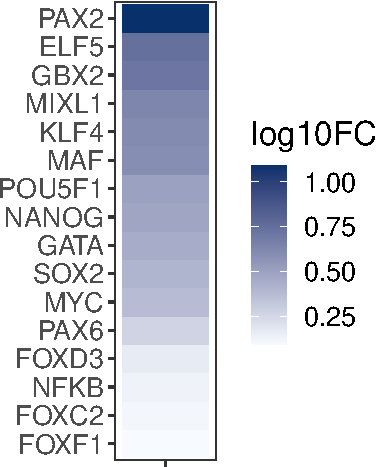
\includegraphics{enrichmotifpairR_user_manual_guide_files/figure-latex/H1_ESC_4-1.pdf}

Now plot the top 10 binding partners for the above TF motifs.

\begin{Shaded}
\begin{Highlighting}[]

\FunctionTok{plotEnrichPair}\NormalTok{(}\AttributeTok{enrich\_pairs =}\NormalTok{ enrich\_motif\_pairs,}
               \AttributeTok{tfs =}\NormalTok{ TF\_list)}
\end{Highlighting}
\end{Shaded}

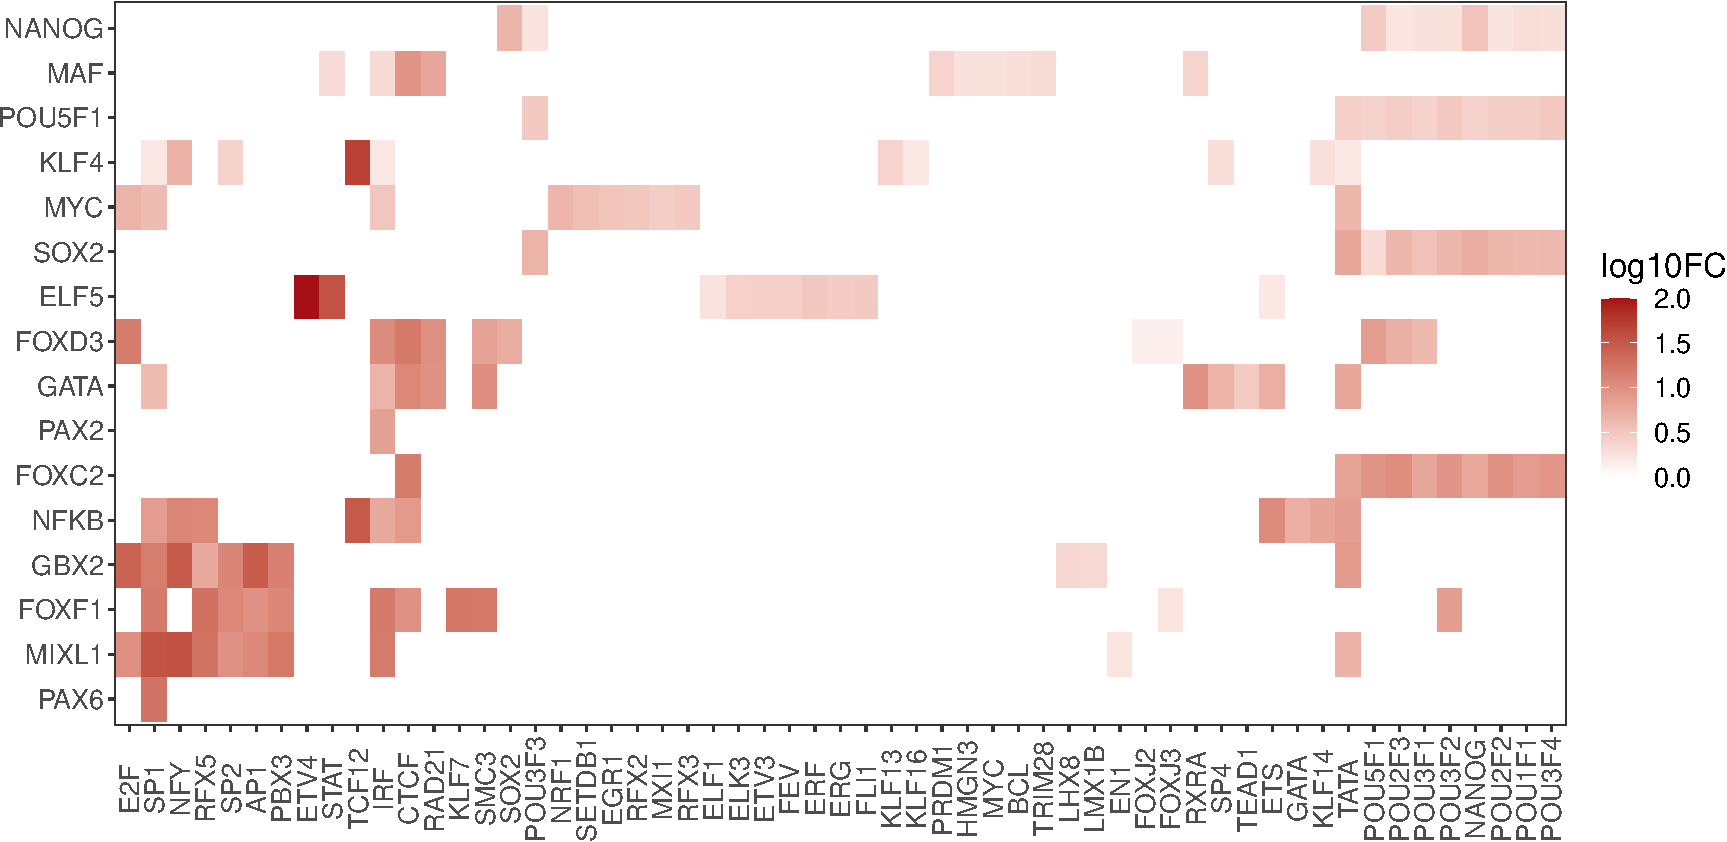
\includegraphics{enrichmotifpairR_user_manual_guide_files/figure-latex/H1_ESC_5-1.pdf}

Now we can make colorful networks for select TFs of interest

\begin{Shaded}
\begin{Highlighting}[]

\CommentTok{\# select TF "SOX2" and extract its connections}
\FunctionTok{plotNetwork}\NormalTok{(}\AttributeTok{enrich\_pairs =}\NormalTok{ enrich\_motif\_pairs, }
            \AttributeTok{TF\_name =} \StringTok{"SOX2"}
\NormalTok{            )}
\end{Highlighting}
\end{Shaded}

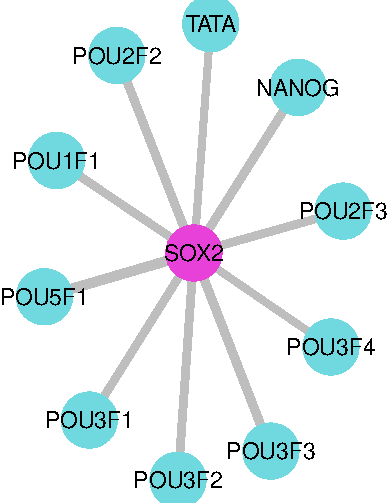
\includegraphics{enrichmotifpairR_user_manual_guide_files/figure-latex/H1_ESC_6-1.pdf}

\begin{Shaded}
\begin{Highlighting}[]

\CommentTok{\# select TF "NANOG" and extract its connections}
\FunctionTok{plotNetwork}\NormalTok{(}\AttributeTok{enrich\_pairs =}\NormalTok{ enrich\_motif\_pairs, }
            \AttributeTok{TF\_name =} \StringTok{"NANOG"}
\NormalTok{            )}
\end{Highlighting}
\end{Shaded}

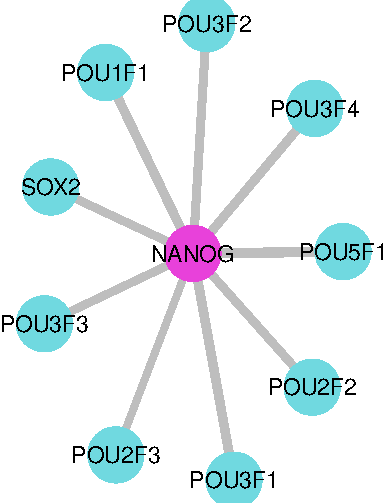
\includegraphics{enrichmotifpairR_user_manual_guide_files/figure-latex/H1_ESC_6-2.pdf}

\begin{Shaded}
\begin{Highlighting}[]

\CommentTok{\# select TF "KLF4" and extract its connections}
\FunctionTok{plotNetwork}\NormalTok{(}\AttributeTok{enrich\_pairs =}\NormalTok{ enrich\_motif\_pairs, }
            \AttributeTok{TF\_name =} \StringTok{"KLF4"}
\NormalTok{            )}
\end{Highlighting}
\end{Shaded}

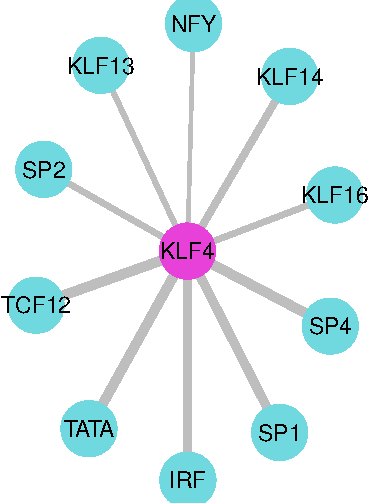
\includegraphics{enrichmotifpairR_user_manual_guide_files/figure-latex/H1_ESC_6-3.pdf}

\hypertarget{additional-example-use-cases}{%
\subsection{Additional example use
cases:}\label{additional-example-use-cases}}

\hypertarget{example-use-case-1-genomic-regions-from-two-conditions}{%
\subsubsection{Example use case 1: Genomic regions from two
conditions}\label{example-use-case-1-genomic-regions-from-two-conditions}}

Here, we have genomic regions from two conditions, for instance, cells
treated vs untreated. To demonstrate this example, we obtained the
ATAC-seq data in Th17 cells treated with a stimulus and untreated Th17
cells. We can find TFs and their binding partner TFs specifically
enriched in stimulated cells relative to untreated cells. To do so, we
need to provide ATAC-seq peaks from stimulated cells as the input set
and ATAC-seq peaks from untreated cells as the control set in the
\texttt{enrichmotifpairR} package.

\begin{Shaded}
\begin{Highlighting}[]
\CommentTok{\# Finding the enriched motifs and their partners}
\NormalTok{results }\OtherTok{\textless{}{-}} \FunctionTok{findEnrichMotifPair}\NormalTok{(}
  \AttributeTok{target\_data =}\NormalTok{ example\_peaks\_data}\SpecialCharTok{$}\NormalTok{Th17\_stimulated\_ATAC\_seq\_peaks,}
  \AttributeTok{background\_data =}\NormalTok{ example\_peaks\_data}\SpecialCharTok{$}\NormalTok{Th17\_ATAC\_seq\_peaks,}
  \AttributeTok{genome\_ver =} \StringTok{"hg19"}\NormalTok{,}
  \AttributeTok{scramble\_data =} \ConstantTok{FALSE}\NormalTok{,}
  \AttributeTok{motif\_database =} \StringTok{"ENCODE"}\NormalTok{,}
  \AttributeTok{Pvalue\_computation =} \StringTok{"hyper"}\NormalTok{,}
  \AttributeTok{Pvalue\_threshold =} \FloatTok{0.05}\NormalTok{,}
  \AttributeTok{Pvalue\_adjust\_method =} \StringTok{"BH"}
\NormalTok{)}
\end{Highlighting}
\end{Shaded}

Assign the resulting data to individual objects and filter motifs for
only TFs genes. TF genes are defined by
\href{https://pubmed.ncbi.nlm.nih.gov/29425488/}{Lambert et al., 2018}.

\begin{Shaded}
\begin{Highlighting}[]
\CommentTok{\# assign the results data to individual objects}
\NormalTok{enrich\_motifs }\OtherTok{\textless{}{-}}\NormalTok{ results}\SpecialCharTok{$}\NormalTok{motif\_enrich}
\NormalTok{enrich\_motif\_pairs }\OtherTok{\textless{}{-}}\NormalTok{ results}\SpecialCharTok{$}\NormalTok{motif\_pair\_enrich}
\end{Highlighting}
\end{Shaded}

\textbf{Plot the heatmap of enriched TF motifs}

\begin{Shaded}
\begin{Highlighting}[]
\CommentTok{\# plot enrichment for list of TF genes}

\FunctionTok{plotEnrichment}\NormalTok{(}\AttributeTok{enrich\_motifs =}\NormalTok{ enrich\_motifs,}
               \AttributeTok{tfs =}\NormalTok{ TF\_list)}
\end{Highlighting}
\end{Shaded}

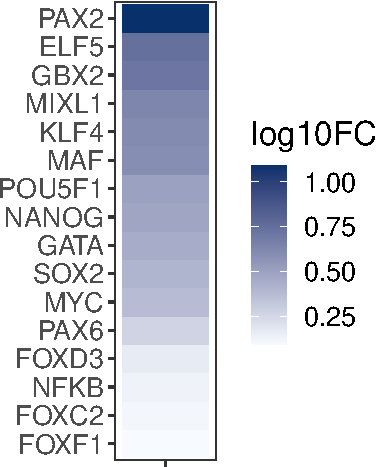
\includegraphics{enrichmotifpairR_user_manual_guide_files/figure-latex/Th17_treated_vs_untreated_4-1.pdf}

\textbf{Now plot the binding partners for the above TF motifs}

\begin{Shaded}
\begin{Highlighting}[]

\FunctionTok{plotEnrichPair}\NormalTok{(}\AttributeTok{enrich\_pairs =}\NormalTok{ enrich\_motif\_pairs,}
               \AttributeTok{tfs =}\NormalTok{ TF\_list)}
\end{Highlighting}
\end{Shaded}

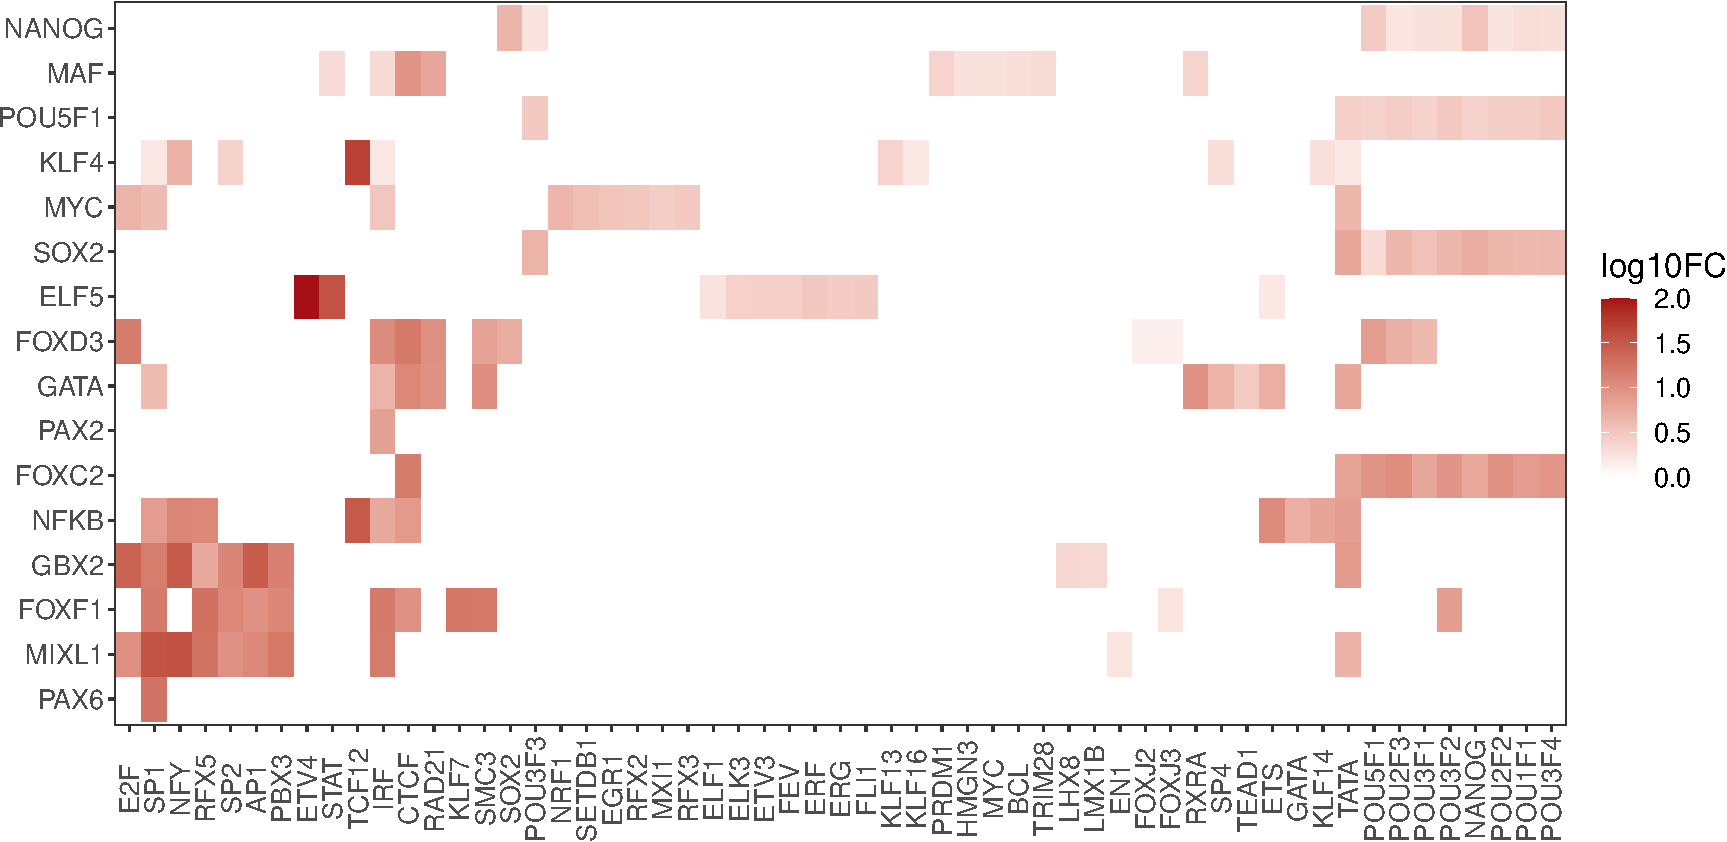
\includegraphics{enrichmotifpairR_user_manual_guide_files/figure-latex/Th17_treated_vs_untreated_5-1.pdf}

Now we can make colorful networks for select TFs of interest.

\begin{Shaded}
\begin{Highlighting}[]
  
\CommentTok{\# select TF "BACH2" and extract its connections}
\FunctionTok{plotNetwork}\NormalTok{(}\AttributeTok{enrich\_pairs =}\NormalTok{ enrich\_motif\_pairs, }
            \AttributeTok{TF\_name =} \StringTok{"BACH2"}
\NormalTok{            )}
\end{Highlighting}
\end{Shaded}

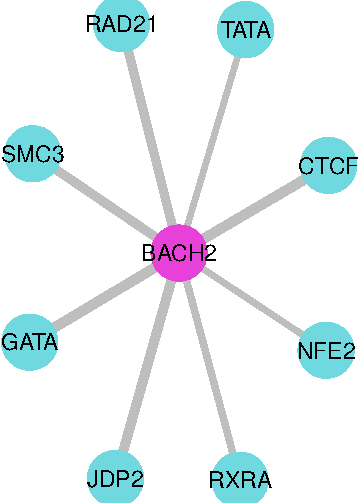
\includegraphics{enrichmotifpairR_user_manual_guide_files/figure-latex/Th17_treated_vs_untreated_6-1.pdf}

\begin{Shaded}
\begin{Highlighting}[]

\CommentTok{\# select TF "TCF12" and extract its connections}
\FunctionTok{plotNetwork}\NormalTok{(}\AttributeTok{enrich\_pairs =}\NormalTok{ enrich\_motif\_pairs, }
            \AttributeTok{TF\_name =} \StringTok{"TCF12"}
\NormalTok{            )}
\end{Highlighting}
\end{Shaded}

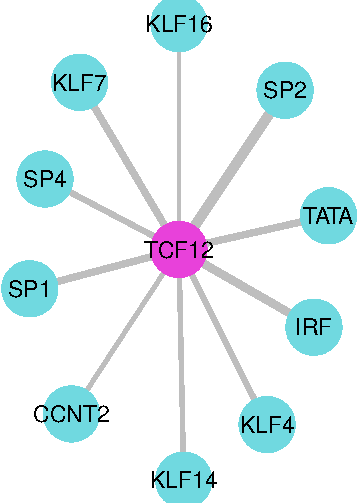
\includegraphics{enrichmotifpairR_user_manual_guide_files/figure-latex/Th17_treated_vs_untreated_6-2.pdf}

\begin{Shaded}
\begin{Highlighting}[]

\CommentTok{\# select TF "HOXA5" and extract its connections}
\FunctionTok{plotNetwork}\NormalTok{(}\AttributeTok{enrich\_pairs =}\NormalTok{ enrich\_motif\_pairs, }
            \AttributeTok{TF\_name =} \StringTok{"HOXA5"}
\NormalTok{            )}
\end{Highlighting}
\end{Shaded}

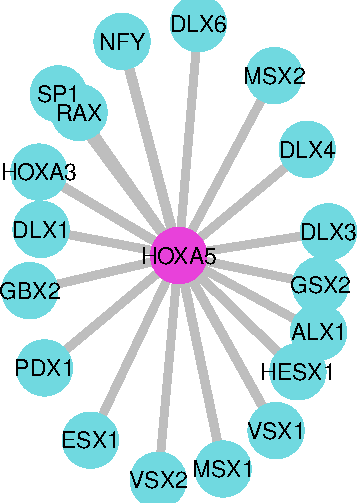
\includegraphics{enrichmotifpairR_user_manual_guide_files/figure-latex/Th17_treated_vs_untreated_6-3.pdf}

\hypertarget{example-use-case-2-genomic-regions-from-two-conditions}{%
\subsubsection{Example use case 2: Genomic regions from two
conditions}\label{example-use-case-2-genomic-regions-from-two-conditions}}

Here, we have genomic regions from two conditions, for instance, cells
differentiating from one cell fate to another. To demonstrate this
example, we obtained ATAC-seq data in Th0 cells (activated T cells)
moving to Th1. We can find TFs and their binding partner TFs
specifically enriched in Th1 cells relative to Th0 cells. To do so, we
need to provide ATAC-seq peaks from Th1 cells as the input set and
ATAC-seq peaks from Th0 cells as the control set in the
\texttt{enrichmotifpairR} package. In this case, we are selecting motifs
from the \texttt{CISBP} database.

\begin{Shaded}
\begin{Highlighting}[]
\CommentTok{\# Finding the enriched motifs and their partners}
\NormalTok{results }\OtherTok{\textless{}{-}} \FunctionTok{findEnrichMotifPair}\NormalTok{(}
  \AttributeTok{target\_data =}\NormalTok{ example\_peaks\_data}\SpecialCharTok{$}\NormalTok{Th1\_ATAC\_seq\_peaks,}
  \AttributeTok{background\_data =}\NormalTok{ example\_peaks\_data}\SpecialCharTok{$}\NormalTok{Th0\_ATAC\_seq\_peaks,}
  \AttributeTok{genome\_ver =} \StringTok{"hg19"}\NormalTok{,}
  \AttributeTok{scramble\_data =} \ConstantTok{FALSE}\NormalTok{,}
  \AttributeTok{motif\_database =} \StringTok{"CISBP"}\NormalTok{,}
  \AttributeTok{Pvalue\_computation =} \StringTok{"hyper"}\NormalTok{,}
  \AttributeTok{Pvalue\_threshold =} \FloatTok{0.01}\NormalTok{,}
  \AttributeTok{Pvalue\_adjust\_method =} \StringTok{"BH"}
\NormalTok{)}
\end{Highlighting}
\end{Shaded}

Assign the resulting data to individual objects and filter motifs for
only TFs genes. TF genes are defined by
\href{https://pubmed.ncbi.nlm.nih.gov/29425488/}{Lambert et al., 2018}.

\begin{Shaded}
\begin{Highlighting}[]
\CommentTok{\# assign the results data to individual objects}
\NormalTok{enrich\_motifs }\OtherTok{\textless{}{-}}\NormalTok{ results}\SpecialCharTok{$}\NormalTok{motif\_enrich}
\NormalTok{enrich\_motif\_pairs }\OtherTok{\textless{}{-}}\NormalTok{ results}\SpecialCharTok{$}\NormalTok{motif\_pair\_enrich}

\NormalTok{TF\_list }\OtherTok{\textless{}{-}} \FunctionTok{unique}\NormalTok{(}\FunctionTok{sort}\NormalTok{(}\FunctionTok{c}\NormalTok{(}\StringTok{"STAT1"}\NormalTok{, }\StringTok{"STAT3"}\NormalTok{, }\StringTok{"STAT4"}\NormalTok{, }\StringTok{"STAT5A"}\NormalTok{, }\StringTok{"STAT5B"}\NormalTok{, }\StringTok{"ATF3"}\NormalTok{, }
                         \StringTok{"JUN"}\NormalTok{, }\StringTok{"JUNB"}\NormalTok{, }\StringTok{"FOXO1"}\NormalTok{, }\StringTok{"HAND1"}\NormalTok{, }\StringTok{"NFATC1"}\NormalTok{, }\StringTok{"NFATC2"}\NormalTok{, }
                         \StringTok{"NFATC3"}\NormalTok{, }\StringTok{"NFATC4"}\NormalTok{, }\StringTok{"SRF"}\NormalTok{, }\StringTok{"RUNX3"}\NormalTok{, }\StringTok{"IRF1"}\NormalTok{, }\StringTok{"IRF6"}\NormalTok{, }
                         \StringTok{"ETV5"}\NormalTok{)))}
\end{Highlighting}
\end{Shaded}

\textbf{Plot the heatmap of enriched TF motifs}

\begin{Shaded}
\begin{Highlighting}[]

\FunctionTok{plotEnrichment}\NormalTok{(}\AttributeTok{enrich\_motifs =}\NormalTok{ enrich\_motifs,}
               \AttributeTok{tfs =}\NormalTok{ TF\_list)}
\end{Highlighting}
\end{Shaded}

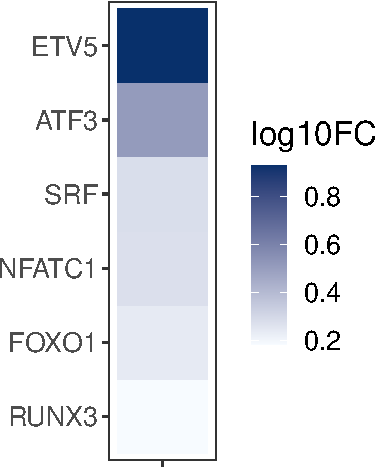
\includegraphics{enrichmotifpairR_user_manual_guide_files/figure-latex/Th1_vs_Th0_4-1.pdf}

Now plot the binding partners for the above TF motifs.

\begin{Shaded}
\begin{Highlighting}[]

\FunctionTok{plotEnrichPair}\NormalTok{(}\AttributeTok{enrich\_pairs =}\NormalTok{ enrich\_motif\_pairs,}
               \AttributeTok{tfs =}\NormalTok{ TF\_list)}
\end{Highlighting}
\end{Shaded}

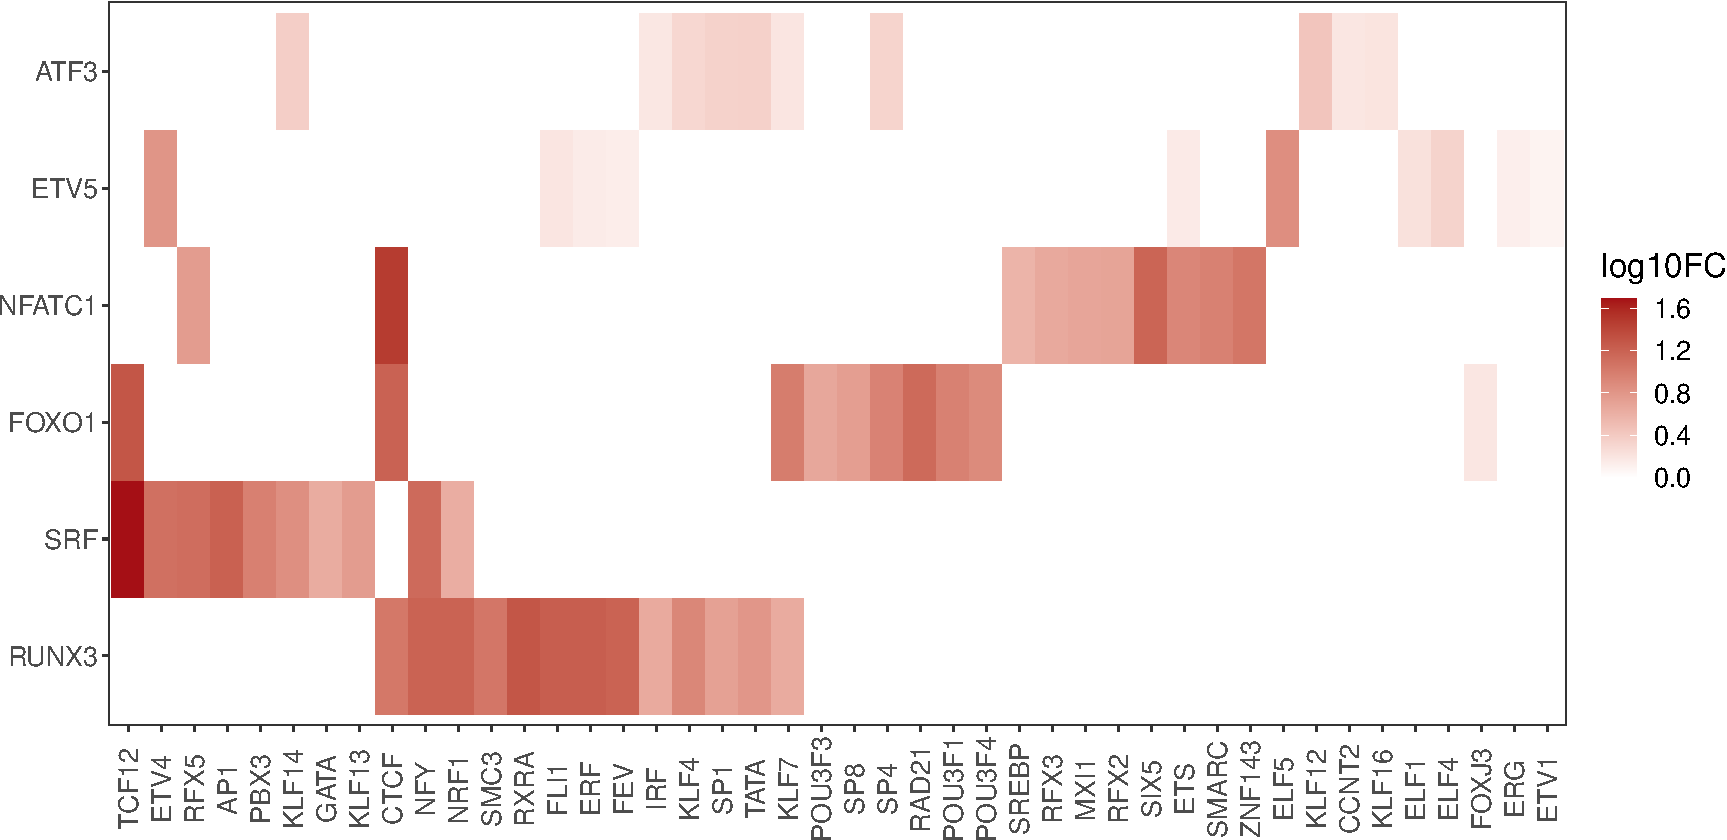
\includegraphics{enrichmotifpairR_user_manual_guide_files/figure-latex/Th1_vs_Th0_5-1.pdf}

\textbf{Now we can make colorful networks for select TFs of interest
using the \texttt{igraph} package}.

\begin{Shaded}
\begin{Highlighting}[]

\CommentTok{\# select TF "NFY" and extract its connections}
\FunctionTok{plotNetwork}\NormalTok{(}\AttributeTok{enrich\_pairs =}\NormalTok{ enrich\_motif\_pairs,}
            \AttributeTok{TF\_name =} \StringTok{"NFY"}
\NormalTok{            )}
\end{Highlighting}
\end{Shaded}

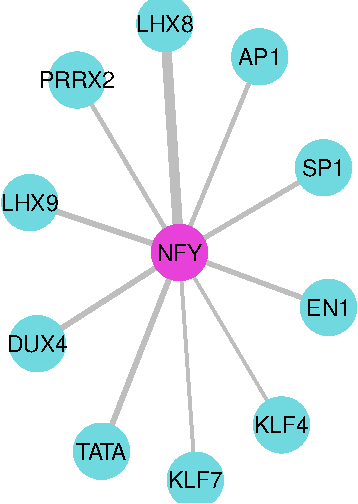
\includegraphics{enrichmotifpairR_user_manual_guide_files/figure-latex/Th1_vs_Th0_6-1.pdf}

\begin{Shaded}
\begin{Highlighting}[]

\CommentTok{\# select TF "HAND1" and extract its connections}
\FunctionTok{plotNetwork}\NormalTok{(}\AttributeTok{enrich\_pairs =}\NormalTok{ enrich\_motif\_pairs,}
            \AttributeTok{TF\_name =} \StringTok{"SMC3"}
\NormalTok{            )}
\CommentTok{\#\textgreater{} Warning in GGally::ggnet2(network, node.size = 12, node.color = my\_color, :}
\CommentTok{\#\textgreater{} ggnet2 does not know how to handle self{-}loops}
\end{Highlighting}
\end{Shaded}

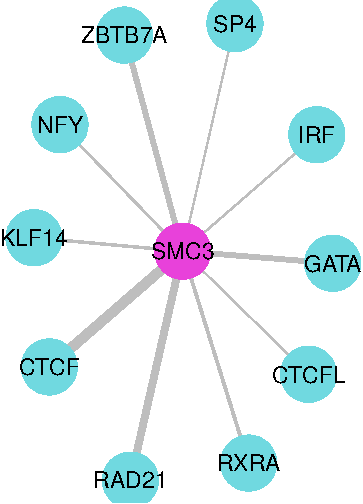
\includegraphics{enrichmotifpairR_user_manual_guide_files/figure-latex/Th1_vs_Th0_6-2.pdf}

\hypertarget{example-use-case-3-genomic-regions-from-two-chromatin-states}{%
\subsubsection{Example use case 3: Genomic regions from two chromatin
states}\label{example-use-case-3-genomic-regions-from-two-chromatin-states}}

Here, we have genomic regions from two chromatin states, for instance,
active genomic regions vs repressive genomic regions. To demonstrate
this example, we obtained H3K27ac peaks representing active regions and
H3K27me3 peaks representing repressive genomic regions in CD8+ cells. We
can find TFs and their binding partner TFs specifically enriched at
active genomic regions relative to repressive regions. To do so, we need
to provide H3K27ac peaks as the input set and H3K27me3 peaks as the
control set in the \texttt{enrichmotifpairR} package. In this case, we
are selecting motifs from the \texttt{JASPAR-CORE} database.

\begin{Shaded}
\begin{Highlighting}[]
\CommentTok{\# Finding the enriched motifs and their partners}
\NormalTok{results }\OtherTok{\textless{}{-}} \FunctionTok{findEnrichMotifPair}\NormalTok{(}
  \AttributeTok{target\_data =}\NormalTok{ example\_peaks\_data}\SpecialCharTok{$}\StringTok{\textasciigrave{}}\AttributeTok{CD8+\_H3K27ac\_peaks}\StringTok{\textasciigrave{}}\NormalTok{,}
  \AttributeTok{background\_data =}\NormalTok{ example\_peaks\_data}\SpecialCharTok{$}\StringTok{\textasciigrave{}}\AttributeTok{CD8+\_H3K27me3\_peaks}\StringTok{\textasciigrave{}}\NormalTok{,}
  \AttributeTok{genome\_ver =} \StringTok{"hg38"}\NormalTok{,}
  \AttributeTok{scramble\_data =} \ConstantTok{FALSE}\NormalTok{,}
  \AttributeTok{motif\_database =} \StringTok{"JASPAR\_CORE"}\NormalTok{,}
  \AttributeTok{Pvalue\_computation =} \StringTok{"hyper"}\NormalTok{,}
  \AttributeTok{Pvalue\_threshold =} \FloatTok{0.01}\NormalTok{,}
  \AttributeTok{Pvalue\_adjust\_method =} \StringTok{"BH"}
\NormalTok{)}
\end{Highlighting}
\end{Shaded}

Assign the resulting data to individual objects and filter motifs for
only TFs genes. TF genes are defined by
\href{https://pubmed.ncbi.nlm.nih.gov/29425488/}{Lambert et al., 2018}.

\begin{Shaded}
\begin{Highlighting}[]
\CommentTok{\# assign the results data to individual objects}
\NormalTok{enrich\_motifs }\OtherTok{\textless{}{-}}\NormalTok{ results}\SpecialCharTok{$}\NormalTok{motif\_enrich}
\NormalTok{enrich\_motif\_pairs }\OtherTok{\textless{}{-}}\NormalTok{ results}\SpecialCharTok{$}\NormalTok{motif\_pair\_enrich}

\NormalTok{TF\_list }\OtherTok{\textless{}{-}} \FunctionTok{unique}\NormalTok{(}\FunctionTok{sort}\NormalTok{(}\FunctionTok{c}\NormalTok{(}\StringTok{"PRDM1"}\NormalTok{, }\StringTok{"TBX21"}\NormalTok{, }\StringTok{"TBX20"}\NormalTok{, }\StringTok{"EOMES"}\NormalTok{, }\StringTok{"BLIMP1"}\NormalTok{, }\StringTok{"ESRRB"}\NormalTok{, }
                         \StringTok{"ID2"}\NormalTok{, }\StringTok{"ID3"}\NormalTok{, }\StringTok{"CEBPB"}\NormalTok{, }\StringTok{"STAT3"}\NormalTok{, }\StringTok{"STAT5"}\NormalTok{, }\StringTok{"STAT6"}\NormalTok{, }
                         \StringTok{"ATF3"}\NormalTok{, }\StringTok{"FOXO1"}\NormalTok{, }\StringTok{"RUNX1"}\NormalTok{, }\StringTok{"RUNX2"}\NormalTok{, }\StringTok{"GATA1"}\NormalTok{, }\StringTok{"GATA2"}\NormalTok{, }
                         \StringTok{"GATA3"}\NormalTok{, }\StringTok{"GATA4"}\NormalTok{, }\StringTok{"BCL6"}\NormalTok{, }\StringTok{"BATF"}\NormalTok{, }\StringTok{"RORA"}\NormalTok{, }\StringTok{"RORC"}\NormalTok{, }
                         \StringTok{"IRF4"}\NormalTok{, }\StringTok{"REL"}\NormalTok{, }\StringTok{"TCF1"}\NormalTok{, }\StringTok{"TCF7"}\NormalTok{, }\StringTok{"IRF4"}\NormalTok{, }\StringTok{"TCF4"}\NormalTok{, }\StringTok{"EBF1"}\NormalTok{, }
                         \StringTok{"MAF"}\NormalTok{, }\StringTok{"ETS2"}\NormalTok{, }\StringTok{"RUNX3"}\NormalTok{)))}
\end{Highlighting}
\end{Shaded}

\textbf{Plot the heatmap of enriched TF motifs}

\begin{Shaded}
\begin{Highlighting}[]
\CommentTok{\# replace very low values so that it is easy to visualize}
\NormalTok{enrich\_motifs[enrich\_motifs }\SpecialCharTok{\textless{}} \FloatTok{1e{-}300}\NormalTok{] }\OtherTok{\textless{}{-}} \FloatTok{1e{-}300}

\FunctionTok{plotEnrichment}\NormalTok{(}\AttributeTok{enrich\_motifs =}\NormalTok{ enrich\_motifs,}
               \AttributeTok{tfs =}\NormalTok{ TF\_list)}
\end{Highlighting}
\end{Shaded}

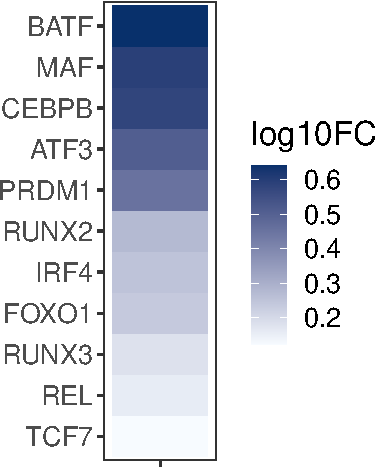
\includegraphics{enrichmotifpairR_user_manual_guide_files/figure-latex/CD8_H3K27ac_vs_H3K27me3_4-1.pdf}

\textbf{Now plot the binding partners for the above TF motifs}

\begin{Shaded}
\begin{Highlighting}[]
\CommentTok{\# replace very low values so that it is easy to visualize}
\NormalTok{enrich\_motif\_pairs[enrich\_motif\_pairs }\SpecialCharTok{\textless{}} \FloatTok{1e{-}100}\NormalTok{] }\OtherTok{\textless{}{-}} \FloatTok{1e{-}100}

\FunctionTok{plotEnrichPair}\NormalTok{(}\AttributeTok{enrich\_pairs =}\NormalTok{ enrich\_motif\_pairs,}
               \AttributeTok{tfs =}\NormalTok{ TF\_list)}
\end{Highlighting}
\end{Shaded}

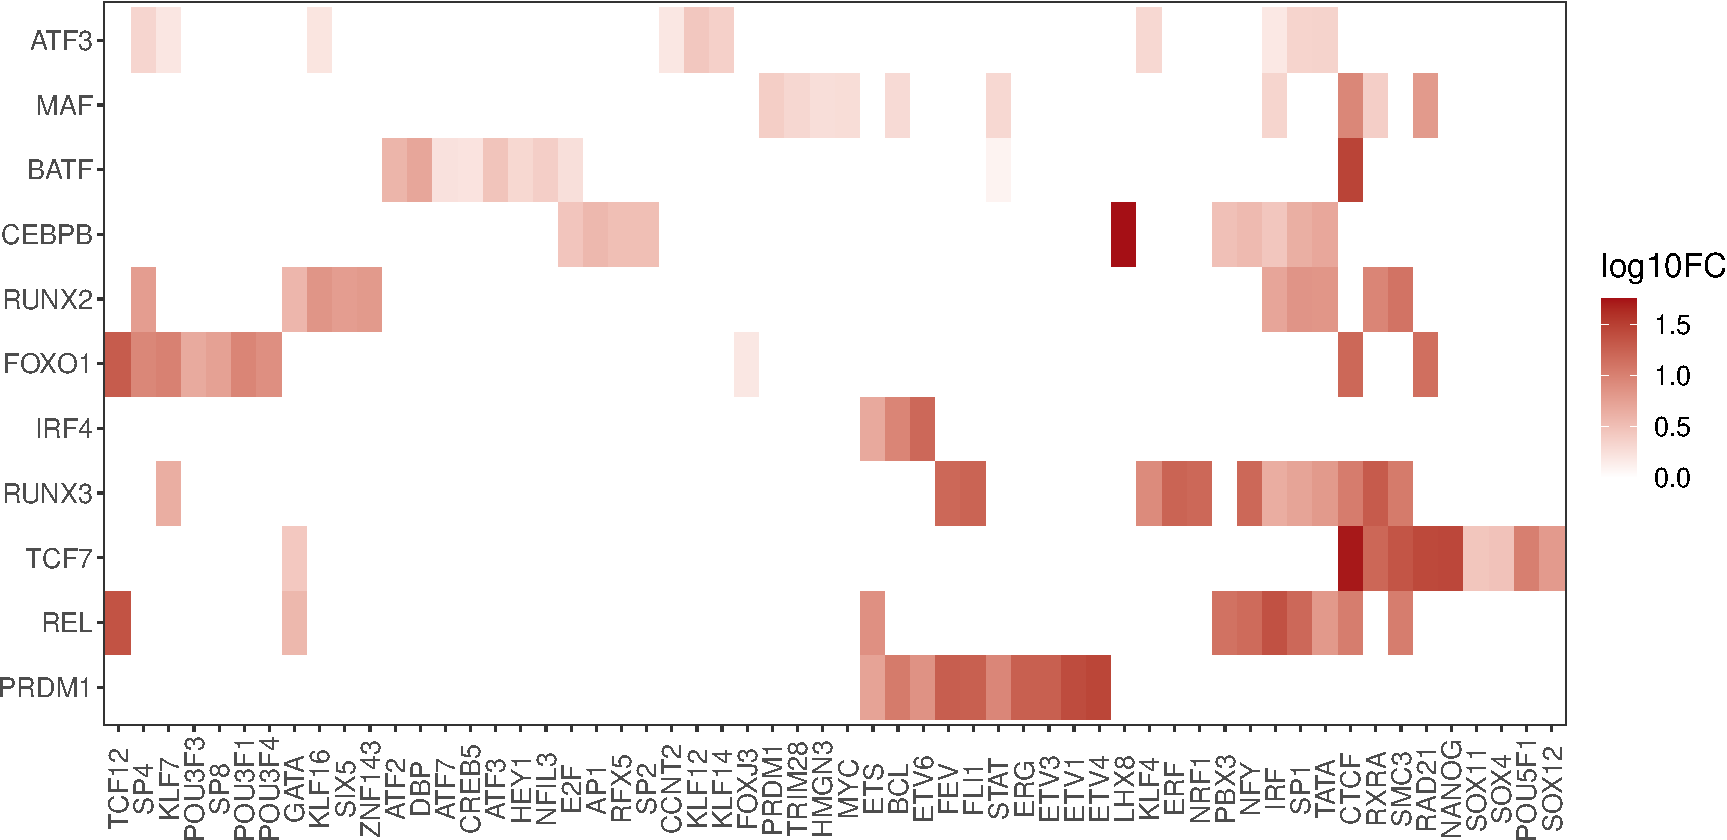
\includegraphics{enrichmotifpairR_user_manual_guide_files/figure-latex/CD8_H3K27ac_vs_H3K27me3_5-1.pdf}

\textbf{Now we can make colorful networks for select TFs of interest
using the \texttt{igraph} package}.

\begin{Shaded}
\begin{Highlighting}[]

\CommentTok{\# select TF "BATF" and extract its connections}
\FunctionTok{plotNetwork}\NormalTok{(}\AttributeTok{enrich\_pairs =}\NormalTok{ enrich\_motif\_pairs, }
            \AttributeTok{TF\_name =} \StringTok{"BATF"}
\NormalTok{            )}
\end{Highlighting}
\end{Shaded}

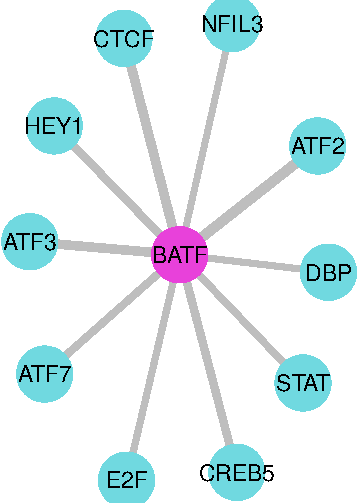
\includegraphics{enrichmotifpairR_user_manual_guide_files/figure-latex/CD8_H3K27ac_vs_H3K27me3_6-1.pdf}

\begin{Shaded}
\begin{Highlighting}[]

\CommentTok{\# select TF "MAF" and extract its connections}
\FunctionTok{plotNetwork}\NormalTok{(}\AttributeTok{enrich\_pairs =}\NormalTok{ enrich\_motif\_pairs, }
            \AttributeTok{TF\_name =} \StringTok{"MAF"}
\NormalTok{            )}
\end{Highlighting}
\end{Shaded}

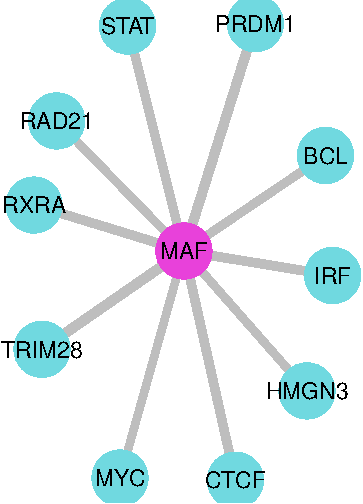
\includegraphics{enrichmotifpairR_user_manual_guide_files/figure-latex/CD8_H3K27ac_vs_H3K27me3_6-2.pdf}

\begin{Shaded}
\begin{Highlighting}[]

\CommentTok{\# select TF "NFKB" and extract its connections}
\FunctionTok{plotNetwork}\NormalTok{(}\AttributeTok{enrich\_pairs =}\NormalTok{ enrich\_motif\_pairs, }
            \AttributeTok{TF\_name =} \StringTok{"NFKB"}
\NormalTok{            )}
\end{Highlighting}
\end{Shaded}

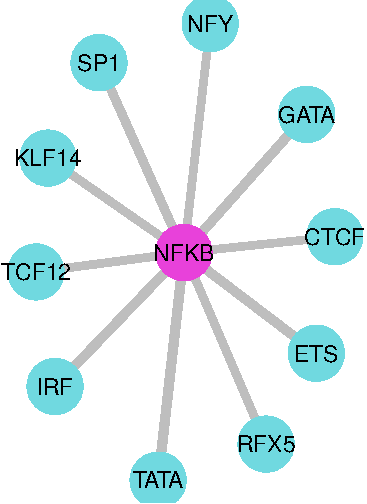
\includegraphics{enrichmotifpairR_user_manual_guide_files/figure-latex/CD8_H3K27ac_vs_H3K27me3_6-3.pdf}

\hypertarget{special-use-cases}{%
\subsection{Special use cases:}\label{special-use-cases}}

\hypertarget{finding-enriched-tf-motif-pairs-from-jolma-et-al.2015.}{%
\subsubsection{\texorpdfstring{Finding enriched TF motif pairs from
\href{https://pubmed.ncbi.nlm.nih.gov/26550823/}{Jolma et
al.,2015}.}{Finding enriched TF motif pairs from Jolma et al.,2015.}}\label{finding-enriched-tf-motif-pairs-from-jolma-et-al.2015.}}

In the paper \href{https://pubmed.ncbi.nlm.nih.gov/26550823/}{Jolma et
al.,2015}, the authors report PWM for pairs of TFs and if you want to
find enrichment of these TF pairs in the input peaks one can use the
function \texttt{findEnrichMotifPair\_Jolma2015}.

Here, we demonstrate this functionality by using genomic regions from
two conditions, for instance, cells differentiating from one cell fate
to another. We obtained ATAC-seq data in Th0 cells (activated T cells)
moving to Th2. We can find enriched TF pairs in Th2 cells relative to
Th0 cells. To do so, we need to provide ATAC-seq peaks from Th2 cells as
the input set and ATAC-seq peaks from Th0 cells as the control set in
the \texttt{enrichmotifpairR} package.

\begin{Shaded}
\begin{Highlighting}[]
\CommentTok{\# Finding the enriched motif pairs}
\NormalTok{results }\OtherTok{\textless{}{-}} \FunctionTok{findEnrichMotifPair\_Jolma2015}\NormalTok{(}
  \AttributeTok{target\_data =}\NormalTok{ example\_peaks\_data}\SpecialCharTok{$}\NormalTok{Th2\_ATAC\_seq\_peaks,}
  \AttributeTok{background\_data =}\NormalTok{ example\_peaks\_data}\SpecialCharTok{$}\NormalTok{Th0\_ATAC\_seq\_peaks,}
  \AttributeTok{genome\_ver =} \StringTok{"hg19"}\NormalTok{,}
  \AttributeTok{scramble\_data =} \ConstantTok{FALSE}\NormalTok{,}
  \AttributeTok{Pvalue\_computation =} \StringTok{"hyper"}\NormalTok{,}
  \AttributeTok{Pvalue\_threshold =} \FloatTok{0.01}\NormalTok{,}
  \AttributeTok{Pvalue\_adjust\_method =} \StringTok{"BH"}
\NormalTok{)}
\end{Highlighting}
\end{Shaded}

The enriched TF motif pairs are stored in the \texttt{results}.

\begin{Shaded}
\begin{Highlighting}[]
\NormalTok{enrich\_motif\_pairs }\OtherTok{\textless{}{-}}\NormalTok{ results}\SpecialCharTok{$}\NormalTok{motif\_pair\_enrich}
\CommentTok{\# The output of the enriched motif pairs }
\NormalTok{enrich\_motif\_pairs[, }\DecValTok{2}\SpecialCharTok{:}\DecValTok{7}\NormalTok{] }\SpecialCharTok{\%\textgreater{}\%} \FunctionTok{head}\NormalTok{(}\DecValTok{10}\NormalTok{) }\SpecialCharTok{\%\textgreater{}\%} 
\NormalTok{    knitr}\SpecialCharTok{::}\FunctionTok{kable}\NormalTok{(., }\AttributeTok{caption=}\StringTok{"Top 10 motif pairs"}\NormalTok{)}
\end{Highlighting}
\end{Shaded}

\begin{longtable}[]{@{}lllrrr@{}}
\caption{Top 10 motif pairs}\tabularnewline
\toprule
TF\_name\_1 & motif\_name\_2 & TF\_name\_2 & fold\_enrich & pval &
pval\_adj \\
\midrule
\endfirsthead
\toprule
TF\_name\_1 & motif\_name\_2 & TF\_name\_2 & fold\_enrich & pval &
pval\_adj \\
\midrule
\endhead
NFY & TATA\_disc6 & TATA & 1.5677851 & 0.00e+00 & 0.00000003 \\
NFY & EN1\_4 & EN1 & 5.8978583 & 0.00e+00 & 0.00000017 \\
NFY & SP1\_disc1 & SP1 & 1.4253158 & 0.00e+00 & 0.00000034 \\
NFY & TATA\_disc4 & TATA & 2.4936559 & 3.90e-07 & 0.00013382 \\
NFY & TCF12\_disc3 & TCF12 & 7.3067911 & 4.80e-07 & 0.00014137 \\
NFY & RFX5\_disc2 & RFX5 & 1.2707848 & 9.10e-07 & 0.00022560 \\
NFY & ESX1\_3 & ESX1 & 4.9542010 & 1.15e-06 & 0.00023781 \\
NFY & MIXL1\_1 & MIXL1 & 15.6293245 & 2.87e-06 & 0.00053861 \\
NFY & LBX2\_3 & LBX2 & 4.0793520 & 6.60e-06 & 0.00113538 \\
NFY & E2F\_disc4 & E2F & 1.3377518 & 1.33e-05 & 0.00211175 \\
\bottomrule
\end{longtable}

\begin{Shaded}
\begin{Highlighting}[]
\CommentTok{\# remove the duplicate motif pairs}
\NormalTok{enrich\_motif\_pairs\_filtered }\OtherTok{\textless{}{-}}\NormalTok{ enrich\_motif\_pairs }\SpecialCharTok{\%\textgreater{}\%} 
\NormalTok{    dplyr}\SpecialCharTok{::}\FunctionTok{group\_by}\NormalTok{(TF\_name\_1, TF\_name\_2) }\SpecialCharTok{\%\textgreater{}\%}
\NormalTok{    dplyr}\SpecialCharTok{::}\FunctionTok{distinct}\NormalTok{(TF\_name\_1, TF\_name\_2, }\AttributeTok{.keep\_all =} \ConstantTok{TRUE}\NormalTok{)}
\NormalTok{enrich\_motif\_pairs\_filtered[, }\DecValTok{2}\SpecialCharTok{:}\DecValTok{7}\NormalTok{] }\SpecialCharTok{\%\textgreater{}\%} \FunctionTok{head}\NormalTok{(}\DecValTok{10}\NormalTok{) }\SpecialCharTok{\%\textgreater{}\%} 
\NormalTok{    knitr}\SpecialCharTok{::}\FunctionTok{kable}\NormalTok{(., }\AttributeTok{caption=}\StringTok{"Top 10 motif pairs after removing duplicates"}\NormalTok{)}
\end{Highlighting}
\end{Shaded}

\begin{longtable}[]{@{}lllrrr@{}}
\caption{Top 10 motif pairs after removing duplicates}\tabularnewline
\toprule
TF\_name\_1 & motif\_name\_2 & TF\_name\_2 & fold\_enrich & pval &
pval\_adj \\
\midrule
\endfirsthead
\toprule
TF\_name\_1 & motif\_name\_2 & TF\_name\_2 & fold\_enrich & pval &
pval\_adj \\
\midrule
\endhead
NFY & TATA\_disc6 & TATA & 1.5677851 & 0.000e+00 & 0.00000003 \\
NFY & EN1\_4 & EN1 & 5.8978583 & 0.000e+00 & 0.00000017 \\
NFY & SP1\_disc1 & SP1 & 1.4253158 & 0.000e+00 & 0.00000034 \\
NFY & TCF12\_disc3 & TCF12 & 7.3067911 & 4.800e-07 & 0.00014137 \\
NFY & RFX5\_disc2 & RFX5 & 1.2707848 & 9.100e-07 & 0.00022560 \\
NFY & ESX1\_3 & ESX1 & 4.9542010 & 1.150e-06 & 0.00023781 \\
NFY & MIXL1\_1 & MIXL1 & 15.6293245 & 2.870e-06 & 0.00053861 \\
NFY & LBX2\_3 & LBX2 & 4.0793520 & 6.600e-06 & 0.00113538 \\
NFY & E2F\_disc4 & E2F & 1.3377518 & 1.330e-05 & 0.00211175 \\
NFY & SP4\_2 & SP4 & 2.2194572 & 1.709e-05 & 0.00251980 \\
\bottomrule
\end{longtable}

\hypertarget{directly-finding-all-possible-enriched-tf-motif-pairs-without-first-looking-for-individual-enriched-motifs.}{%
\subsubsection{Directly finding all possible enriched TF motif pairs
without first looking for individual enriched
motifs.}\label{directly-finding-all-possible-enriched-tf-motif-pairs-without-first-looking-for-individual-enriched-motifs.}}

If users are interested in finding all possible enriched TF motif pairs
without first looking for individual enriched motifs, one can use the
function \texttt{findEnrichMotifPairAll}.

Here, we demonstrate this functionality by using genomic regions from
two conditions, for instance, cells differentiating from one cell fate
to another. We obtained ATAC-seq data in Th0 cells (activated T cells)
moving to Th1. We can find all enriched TFs pairs in Th1 cells relative
to Th0 cells. To do so, we need to provide ATAC-seq peaks from Th1 cells
as the input set and ATAC-seq peaks from Th0 cells as the control set in
the \texttt{enrichmotifpairR} package. In this case, we are selecting
motifs from \texttt{JASPAR-UNVALIDATED} database.

\begin{Shaded}
\begin{Highlighting}[]
\CommentTok{\# Finding the enriched motifs and their partners}
\NormalTok{results }\OtherTok{\textless{}{-}} \FunctionTok{findEnrichMotifPairAll}\NormalTok{(}
  \AttributeTok{target\_data =}\NormalTok{ example\_peaks\_data}\SpecialCharTok{$}\NormalTok{Th1\_ATAC\_seq\_peaks,}
  \AttributeTok{background\_data =}\NormalTok{ example\_peaks\_data}\SpecialCharTok{$}\NormalTok{Th0\_ATAC\_seq\_peaks,}
  \AttributeTok{genome\_ver =} \StringTok{"hg19"}\NormalTok{,}
  \AttributeTok{scramble\_data =} \ConstantTok{FALSE}\NormalTok{,}
  \AttributeTok{motif\_database =} \StringTok{"JASPAR\_UNVALIDATED"}\NormalTok{,}
  \AttributeTok{Pvalue\_computation =} \StringTok{"hyper"}\NormalTok{,}
  \AttributeTok{Pvalue\_threshold =} \FloatTok{0.01}\NormalTok{,}
  \AttributeTok{Pvalue\_adjust\_method =} \StringTok{"BH"}
\NormalTok{)}
\end{Highlighting}
\end{Shaded}

The enriched TF motif pairs are stored in the \texttt{results}. These
pairs contain duplicates (redundant entries) and should be removed. To
do so one can make use of the function \texttt{removeDuplicateTFPairs}.
Also filter for only TF genes. TF genes are defined by
\href{https://pubmed.ncbi.nlm.nih.gov/29425488/}{Lambert et al., 2018}.

\begin{Shaded}
\begin{Highlighting}[]
\CommentTok{\# assign the results data to individual objects}
\NormalTok{enrich\_motif\_pairs }\OtherTok{\textless{}{-}}\NormalTok{ results}\SpecialCharTok{$}\NormalTok{motif\_pair\_enrich}
\CommentTok{\# remove duplicate pairs}
\NormalTok{removeDuplicateTFPairs }\OtherTok{\textless{}{-}} \ControlFlowTok{function}\NormalTok{(}\AttributeTok{data =}\NormalTok{ data)\{}
\NormalTok{    data }\OtherTok{\textless{}{-}}\NormalTok{ data }\SpecialCharTok{\%\textgreater{}\%}\NormalTok{ dplyr}\SpecialCharTok{::}\FunctionTok{arrange}\NormalTok{(pval\_adj) }\SpecialCharTok{\%\textgreater{}\%}
\NormalTok{        dplyr}\SpecialCharTok{::}\FunctionTok{mutate}\NormalTok{(}\AttributeTok{key =} \FunctionTok{paste0}\NormalTok{(}\FunctionTok{pmin}\NormalTok{(TF\_name\_1, TF\_name\_2), }
                                   \FunctionTok{pmax}\NormalTok{(TF\_name\_1, TF\_name\_2), }\AttributeTok{sep =} \StringTok{""}\NormalTok{)) }\SpecialCharTok{\%\textgreater{}\%} 
\NormalTok{        dplyr}\SpecialCharTok{::}\FunctionTok{distinct}\NormalTok{(key, }\AttributeTok{.keep\_all =} \ConstantTok{TRUE}\NormalTok{) }\SpecialCharTok{\%\textgreater{}\%} 
\NormalTok{        dplyr}\SpecialCharTok{::}\FunctionTok{filter}\NormalTok{(TF\_name\_1 }\SpecialCharTok{!=}\NormalTok{ TF\_name\_2) }\SpecialCharTok{\%\textgreater{}\%}
\NormalTok{        dplyr}\SpecialCharTok{::}\FunctionTok{select}\NormalTok{(}\SpecialCharTok{{-}}\NormalTok{key)}
    \FunctionTok{return}\NormalTok{(data)}
\NormalTok{\}}
\NormalTok{enrich\_motif\_pairs }\OtherTok{\textless{}{-}} \FunctionTok{removeDuplicateTFPairs}\NormalTok{(}\AttributeTok{data =}\NormalTok{ enrich\_motif\_pairs)}
\CommentTok{\# get the list of TFs genes}
\NormalTok{TF\_df }\OtherTok{\textless{}{-}}\NormalTok{ TF\_df }\SpecialCharTok{\%\textgreater{}\%}\NormalTok{ dplyr}\SpecialCharTok{::}\FunctionTok{filter}\NormalTok{(TF\_Yes\_No }\SpecialCharTok{==} \StringTok{"Yes"}\NormalTok{)}
\CommentTok{\# filter TFs motifs for only TFs genes based on Lambert et al., 2018}
\NormalTok{enrich\_motif\_pairs\_filtered }\OtherTok{\textless{}{-}}\NormalTok{ enrich\_motif\_pairs }\SpecialCharTok{\%\textgreater{}\%} 
\NormalTok{    dplyr}\SpecialCharTok{::}\FunctionTok{distinct}\NormalTok{(TF\_name\_1, TF\_name\_2, }\AttributeTok{.keep\_all =} \ConstantTok{TRUE}\NormalTok{) }\SpecialCharTok{\%\textgreater{}\%} 
\NormalTok{    dplyr}\SpecialCharTok{::}\FunctionTok{filter}\NormalTok{(TF\_name\_1 }\SpecialCharTok{\%in\%}\NormalTok{ TF\_df}\SpecialCharTok{$}\NormalTok{Name) }\SpecialCharTok{\%\textgreater{}\%}
\NormalTok{    dplyr}\SpecialCharTok{::}\FunctionTok{filter}\NormalTok{(TF\_name\_2 }\SpecialCharTok{\%in\%}\NormalTok{ TF\_df}\SpecialCharTok{$}\NormalTok{Name) }\SpecialCharTok{\%\textgreater{}\%}
\NormalTok{    dplyr}\SpecialCharTok{::}\FunctionTok{filter}\NormalTok{(pval\_adj }\SpecialCharTok{\textless{}} \FloatTok{1e{-}05}\NormalTok{)}
\end{Highlighting}
\end{Shaded}

Compare these TF motif pairs with the motif pairs from the functionality
of \texttt{findEnrichMotifPair}.

\begin{Shaded}
\begin{Highlighting}[]
\CommentTok{\# Finding the enriched motifs and their partners}
\NormalTok{results }\OtherTok{\textless{}{-}} \FunctionTok{findEnrichMotifPair}\NormalTok{(}
  \AttributeTok{target\_data =}\NormalTok{ example\_peaks\_data}\SpecialCharTok{$}\NormalTok{Th1\_ATAC\_seq\_peaks,}
  \AttributeTok{background\_data =}\NormalTok{ example\_peaks\_data}\SpecialCharTok{$}\NormalTok{Th0\_ATAC\_seq\_peaks,}
  \AttributeTok{genome\_ver =} \StringTok{"hg19"}\NormalTok{,}
  \AttributeTok{scramble\_data =} \ConstantTok{FALSE}\NormalTok{,}
  \AttributeTok{motif\_database =} \StringTok{"JASPAR\_UNVALIDATED"}\NormalTok{,}
  \AttributeTok{Pvalue\_computation =} \StringTok{"hyper"}\NormalTok{,}
  \AttributeTok{Pvalue\_threshold =} \FloatTok{0.01}\NormalTok{,}
  \AttributeTok{Pvalue\_adjust\_method =} \StringTok{"BH"}
\NormalTok{)}
\end{Highlighting}
\end{Shaded}

\begin{Shaded}
\begin{Highlighting}[]
\CommentTok{\# assign the results data to individual objects}
\NormalTok{enrich\_motif\_pairs\_2 }\OtherTok{\textless{}{-}}\NormalTok{ results}\SpecialCharTok{$}\NormalTok{motif\_pair\_enrich}
\CommentTok{\# remove duplicate pairs}
\NormalTok{removeDuplicateTFPairs }\OtherTok{\textless{}{-}} \ControlFlowTok{function}\NormalTok{(}\AttributeTok{data =}\NormalTok{ data)\{}
\NormalTok{    data }\OtherTok{\textless{}{-}}\NormalTok{ data }\SpecialCharTok{\%\textgreater{}\%}\NormalTok{ dplyr}\SpecialCharTok{::}\FunctionTok{arrange}\NormalTok{(pval\_adj) }\SpecialCharTok{\%\textgreater{}\%}
\NormalTok{        dplyr}\SpecialCharTok{::}\FunctionTok{mutate}\NormalTok{(}\AttributeTok{key =} \FunctionTok{paste0}\NormalTok{(}\FunctionTok{pmin}\NormalTok{(TF\_name\_1, TF\_name\_2), }
                                   \FunctionTok{pmax}\NormalTok{(TF\_name\_1, TF\_name\_2), }\AttributeTok{sep =} \StringTok{""}\NormalTok{)) }\SpecialCharTok{\%\textgreater{}\%} 
\NormalTok{        dplyr}\SpecialCharTok{::}\FunctionTok{distinct}\NormalTok{(key, }\AttributeTok{.keep\_all =} \ConstantTok{TRUE}\NormalTok{) }\SpecialCharTok{\%\textgreater{}\%} 
\NormalTok{        dplyr}\SpecialCharTok{::}\FunctionTok{filter}\NormalTok{(TF\_name\_1 }\SpecialCharTok{!=}\NormalTok{ TF\_name\_2) }\SpecialCharTok{\%\textgreater{}\%}
\NormalTok{        dplyr}\SpecialCharTok{::}\FunctionTok{select}\NormalTok{(}\SpecialCharTok{{-}}\NormalTok{key)}
    \FunctionTok{return}\NormalTok{(data)}
\NormalTok{\}}
\NormalTok{enrich\_motif\_pairs\_2 }\OtherTok{\textless{}{-}} \FunctionTok{removeDuplicateTFPairs}\NormalTok{(}\AttributeTok{data =}\NormalTok{ enrich\_motif\_pairs\_2)}
\CommentTok{\# get the list of TFs genes}
\NormalTok{TF\_df }\OtherTok{\textless{}{-}}\NormalTok{ TF\_df }\SpecialCharTok{\%\textgreater{}\%}\NormalTok{ dplyr}\SpecialCharTok{::}\FunctionTok{filter}\NormalTok{(TF\_Yes\_No }\SpecialCharTok{==} \StringTok{"Yes"}\NormalTok{)}
\CommentTok{\# filter TFs motifs for only TFs genes based on Lambert et al., 2018}
\NormalTok{enrich\_motif\_pairs\_filtered\_2 }\OtherTok{\textless{}{-}}\NormalTok{ enrich\_motif\_pairs\_2 }\SpecialCharTok{\%\textgreater{}\%} 
\NormalTok{    dplyr}\SpecialCharTok{::}\FunctionTok{distinct}\NormalTok{(TF\_name\_1, TF\_name\_2, }\AttributeTok{.keep\_all =} \ConstantTok{TRUE}\NormalTok{) }\SpecialCharTok{\%\textgreater{}\%} 
\NormalTok{    dplyr}\SpecialCharTok{::}\FunctionTok{filter}\NormalTok{(TF\_name\_1 }\SpecialCharTok{\%in\%}\NormalTok{ TF\_df}\SpecialCharTok{$}\NormalTok{Name) }\SpecialCharTok{\%\textgreater{}\%}
\NormalTok{    dplyr}\SpecialCharTok{::}\FunctionTok{filter}\NormalTok{(TF\_name\_2 }\SpecialCharTok{\%in\%}\NormalTok{ TF\_df}\SpecialCharTok{$}\NormalTok{Name) }\SpecialCharTok{\%\textgreater{}\%}
\NormalTok{    dplyr}\SpecialCharTok{::}\FunctionTok{filter}\NormalTok{(pval\_adj }\SpecialCharTok{\textless{}} \FloatTok{1e{-}05}\NormalTok{)}
\end{Highlighting}
\end{Shaded}

\textbf{Comparison plot}

\begin{Shaded}
\begin{Highlighting}[]
\CommentTok{\# create data frame to plot the number of TF pairs comparison plot}
\NormalTok{data }\OtherTok{\textless{}{-}} \FunctionTok{data.frame}\NormalTok{(}\AttributeTok{functionality =} \FunctionTok{c}\NormalTok{(}\StringTok{"findEnrichMotifPair"}\NormalTok{, }\StringTok{"findEnrichMotifPairAll"}\NormalTok{), }\AttributeTok{value =} \FunctionTok{c}\NormalTok{(}\FunctionTok{nrow}\NormalTok{(enrich\_motif\_pairs\_filtered\_2), }\FunctionTok{nrow}\NormalTok{(enrich\_motif\_pairs\_filtered)))}

\CommentTok{\# bar plot}
\NormalTok{pp }\OtherTok{\textless{}{-}} \FunctionTok{ggplot}\NormalTok{(}\AttributeTok{data =}\NormalTok{ data, }
             \FunctionTok{aes}\NormalTok{(}\AttributeTok{x =}\NormalTok{ functionality, }\AttributeTok{y =}\NormalTok{ value, }\AttributeTok{fill =}\NormalTok{ functionality)) }\SpecialCharTok{+} 
    \FunctionTok{geom\_bar}\NormalTok{(}\AttributeTok{stat =} \StringTok{"identity"}\NormalTok{) }\SpecialCharTok{+} 
    \FunctionTok{ylab}\NormalTok{(}\StringTok{""}\NormalTok{) }\SpecialCharTok{+} \FunctionTok{xlab}\NormalTok{(}\StringTok{""}\NormalTok{) }\SpecialCharTok{+} \FunctionTok{theme\_bw}\NormalTok{() }\SpecialCharTok{+} 
    \FunctionTok{theme}\NormalTok{(}\AttributeTok{plot.background =} \FunctionTok{element\_blank}\NormalTok{()}
\NormalTok{    ,}\AttributeTok{panel.grid.major =} \FunctionTok{element\_blank}\NormalTok{()}
\NormalTok{    ,}\AttributeTok{panel.grid.minor =} \FunctionTok{element\_blank}\NormalTok{()}
\NormalTok{    ,}\AttributeTok{text =} \FunctionTok{element\_text}\NormalTok{(}\AttributeTok{size=}\DecValTok{16}\NormalTok{), }\AttributeTok{axis.text.x =} \FunctionTok{element\_text}\NormalTok{(}\AttributeTok{angle=}\DecValTok{90}\NormalTok{, }\AttributeTok{vjust=}\FloatTok{0.5}\NormalTok{)}
\NormalTok{)}
\NormalTok{pp}
\end{Highlighting}
\end{Shaded}

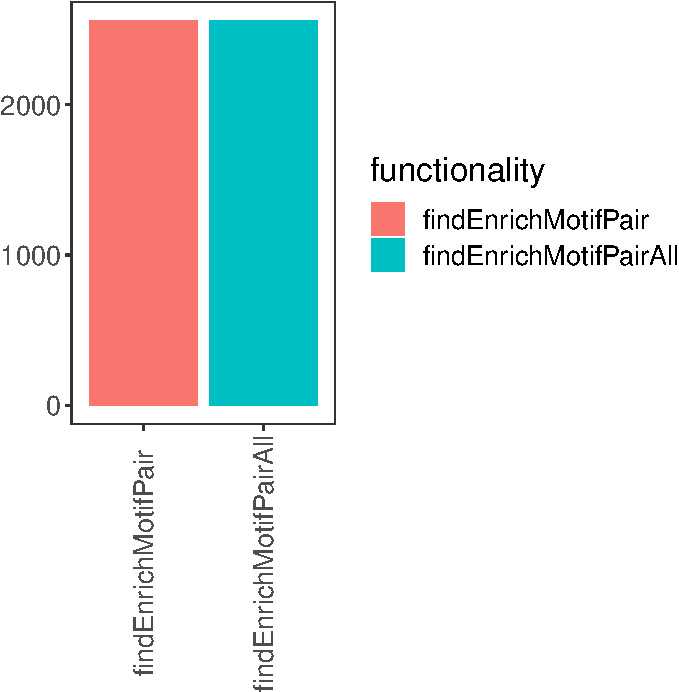
\includegraphics{enrichmotifpairR_user_manual_guide_files/figure-latex/Th1_vs_Th0_all_pairs_3_comparison_plot-1.pdf}

As you can see, \texttt{findEnrichMotifPair} determines relatively fewer
enriched motif pairs than \texttt{findEnrichMotifPairAll}, as the former
finds only the pairs associated with individually enriched motifs.

\end{document}
